\documentclass{tufte-handout}
\usepackage{graphicx}
\usepackage{xcolor}
\graphicspath{ {./images/} }
\title{Dimensionality Reduction}
\author{Andr\'es Ponce}

\begin{document}
\maketitle
\begin{abstract}
Some problems inherently can be modeled using less dimensions
than migth appear at first sight. Taking the well-known digit
recognition problem, even though a sample image might consist of 
100x100 pixels,any digiit on the image can only be transformed by 
rotation,translation, and scaling. We can study this pattern further.
\end{abstract}
\section{Principal Component Analysis}
\textbf{Principal Component Analysis} (PCA) is a poular way of reducing 
dimensions in a given problem by attempting to find a lower dimensional
space on which to map the data points.

\begin{marginfigure}
	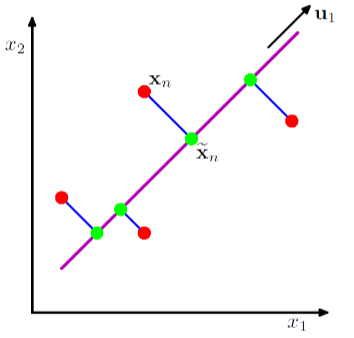
\includegraphics[scale=0.4]{pca}
	\caption{For original dimensions $x_{1}$ and $x_{2}$,  the \textcolor{magenta}{line}
		is the new space we want to map onto. We minimize the sum of the projections of the 
		\textcolor{red}{data point} onto the line, which is at the \textcolor{green}{dot}}
\end{marginfigure}

However, we can also think of PCA as the projection of the points onto a plane such that their
\textit{variance} is maximized.\footnote{This seems similar to a \textbf{linear discriminant}?}
Similar to a linear discriminant, we want to maximize the variance when we project it onto a 
smaller subspace. This will make it so that the points overlap less when brought down to the same line.
Then we have the \textbf{data mean} and the \textbf{projected data mean}
\begin{equation}
\overline{x} = \frac{1}{N}\sum_{n=1}^{N}x_{n}\quad\mathrm{and}\quad u_{1}^{T}\overline{x}
\end{equation}
Where $u$ refers to the mean once the data is projected onto the line.

Finally, the \textbf{covariance matrix} refers to \footnote{So, basically the amount the projected
data and the regular data differ squared, and then take the mean?}
\[ S = \frac{1}{N}\sum_{n=1}^{N}(x_{n} - \overline{x})(x_{n} - \overline{x})^{T}\]

The covariance then tells us how the values of the projected data and the regular data differ. 
\subsection{Lagrangian Multipliers}
To remind, \textbf{Lagrangian Multipliers} allow us to solve \textbf{constrained optimization}. Basically,
we want to optimize an equation subject to a set of constraints. In this case, we have the unit direction vectors
in $M$ dimensional space $u$, so $u_{1}^{T}u_{1} = 1$. This equation acts as our constraint in this case,
\footnote{is this because the covariance can be at most 1?}. And the equation we are then trying to optimize
becomes $u^{T}_{1}Su_{1}$.  

To conclude discussion on PCA, we have to do
\begin{enumerate}
		\item{Find te mean $\overline{x}$ and covariance matrix $S$}
		\item{Find the $M$ eigenvectors of $S$ corresponding to the M largest eigenvalues}
\end{enumerate}
The	eigenvector decomposition takes $O(D^{3})$ and finding the M largest eigenvectors and eigenvalues 
takes $O(MD^{2})$
\section{Minimum Error Formulation}
We are still trying to bring down the original dimensionality to a lower level, and we introduce another 
method called the \textbf{Mininmum Error Formulation}. This approach again reduces a space to another 
$M$ dimensional space. 

Originally, we can have $D$ \textbf{orthonormal}\footnote{Two vectors are \textbf{orthonormal} if they are
both orthogonal(i.e. perpendicular) and unit vectors.} vectors. We then express any position in $D$ dimensions
as a linear combination of the $D$ orhtonormal vectors. Our goal is to then express those same points with a
linear combination of $M$ vectors instead, which would be equivalent to projecting the vectors onto a smaller
subspace.

Then, for this approach to work, if we are to use only $M$ eigenvectors in subspace $u$, we would still need to
perform the decomposition since we would need to find the largest $M$ eigenvectors. Then the approximate point
$\tilde{x}_{n}$ can be written as
\[ \tilde{x}_{n} = \overline{x} + \sum_{i=1}^{M}(x^{T}_{n}u_{i} - \overline{x}^{T}u_{i})u_{i}\]

\begin{center}
	\begin{figure}
		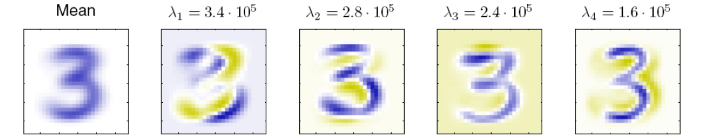
\includegraphics[scale=0.4]{number_class}
		\caption{Here, we take the mean, and we calculate the four PCA eigenvectors, and their 
			corresponding eigenvalues, and calculate their covariance from the mean.}
	\end{figure}
\end{center}
\end{document}

